\documentclass[11pt]{article}
%\usepackage{psfig}
\usepackage{graphicx}
\usepackage{enumitem}
\usepackage{amsmath,amssymb,amsthm,listings,hyperref}
\usepackage{tikz}
\usepackage{latexsym}
\usepackage{amsfonts}

\title{CS 4641 Project 4 Report}
\author{HU Heng}
\begin{document}
\maketitle
\section{Overview}
This report is for CS 4641 Machine Learning project 4 Markov Decision Process. In the following pages, you will see the solution to the chosen Markov decision process using value iteration, policy iteration and Q learning. I will show the convergence of value iteration and policy iteration as well as the influence of changing PJOG values. Finally, Q learning is discussed.

\section{My MDP Problems}
In this project, I use the RL\_sim which is the java executable created by Carnegie Mellon University associates Rohit Kelkar and Vivek Mehta. The problems I would like to solve are both mazes given by the author. Fig.\ref{Fig:maze1} is a very simple 6x9 maze and Fig.\ref{Fig:maze2} is a more complicated 10x10 maze.
\begin{figure}[!htb]
   \begin{minipage}{0.4\textwidth}
     \centering
     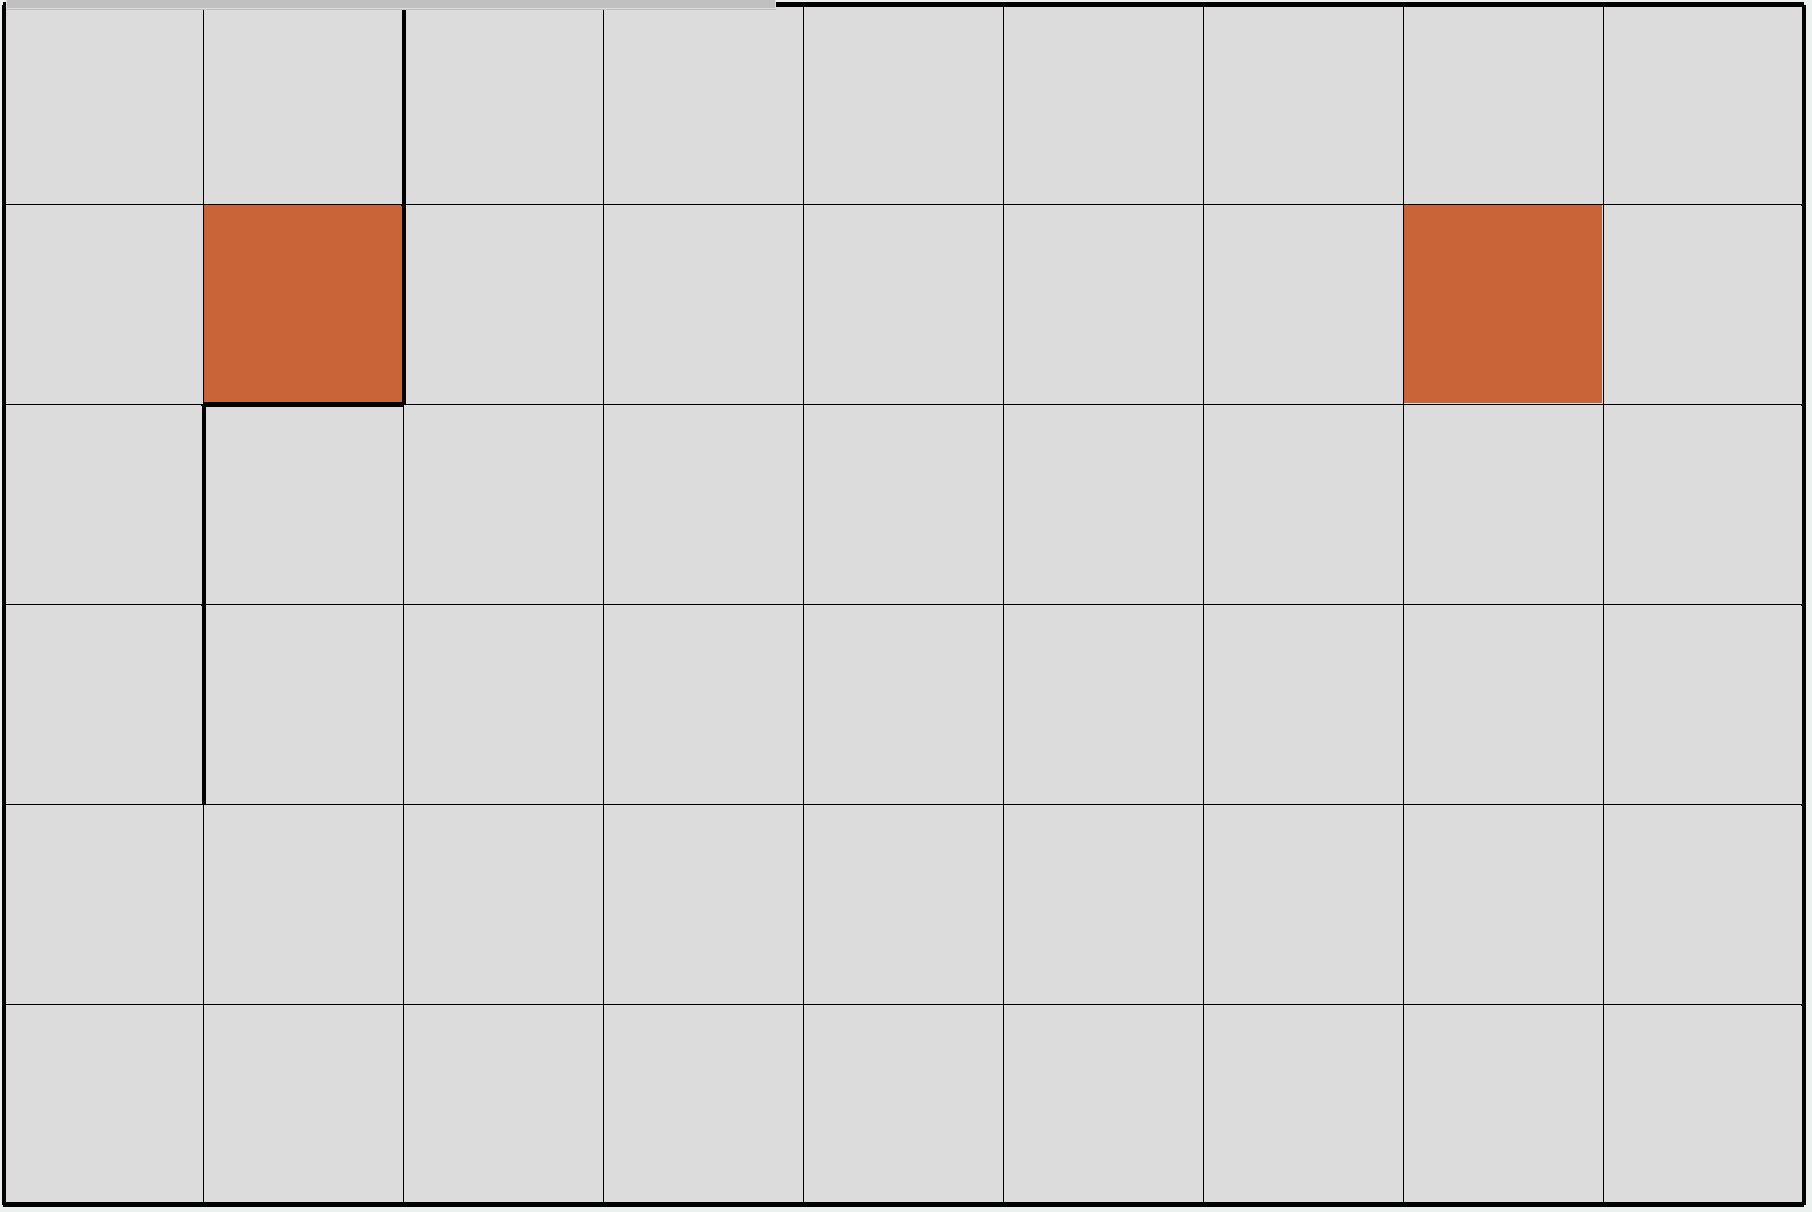
\includegraphics[width=1.2\linewidth]{../figures/maze1.png}
     \caption{Simple Maze}\label{Fig:maze1}
   \end{minipage}\hfill
   \begin{minipage}{0.4\textwidth}
     \centering
     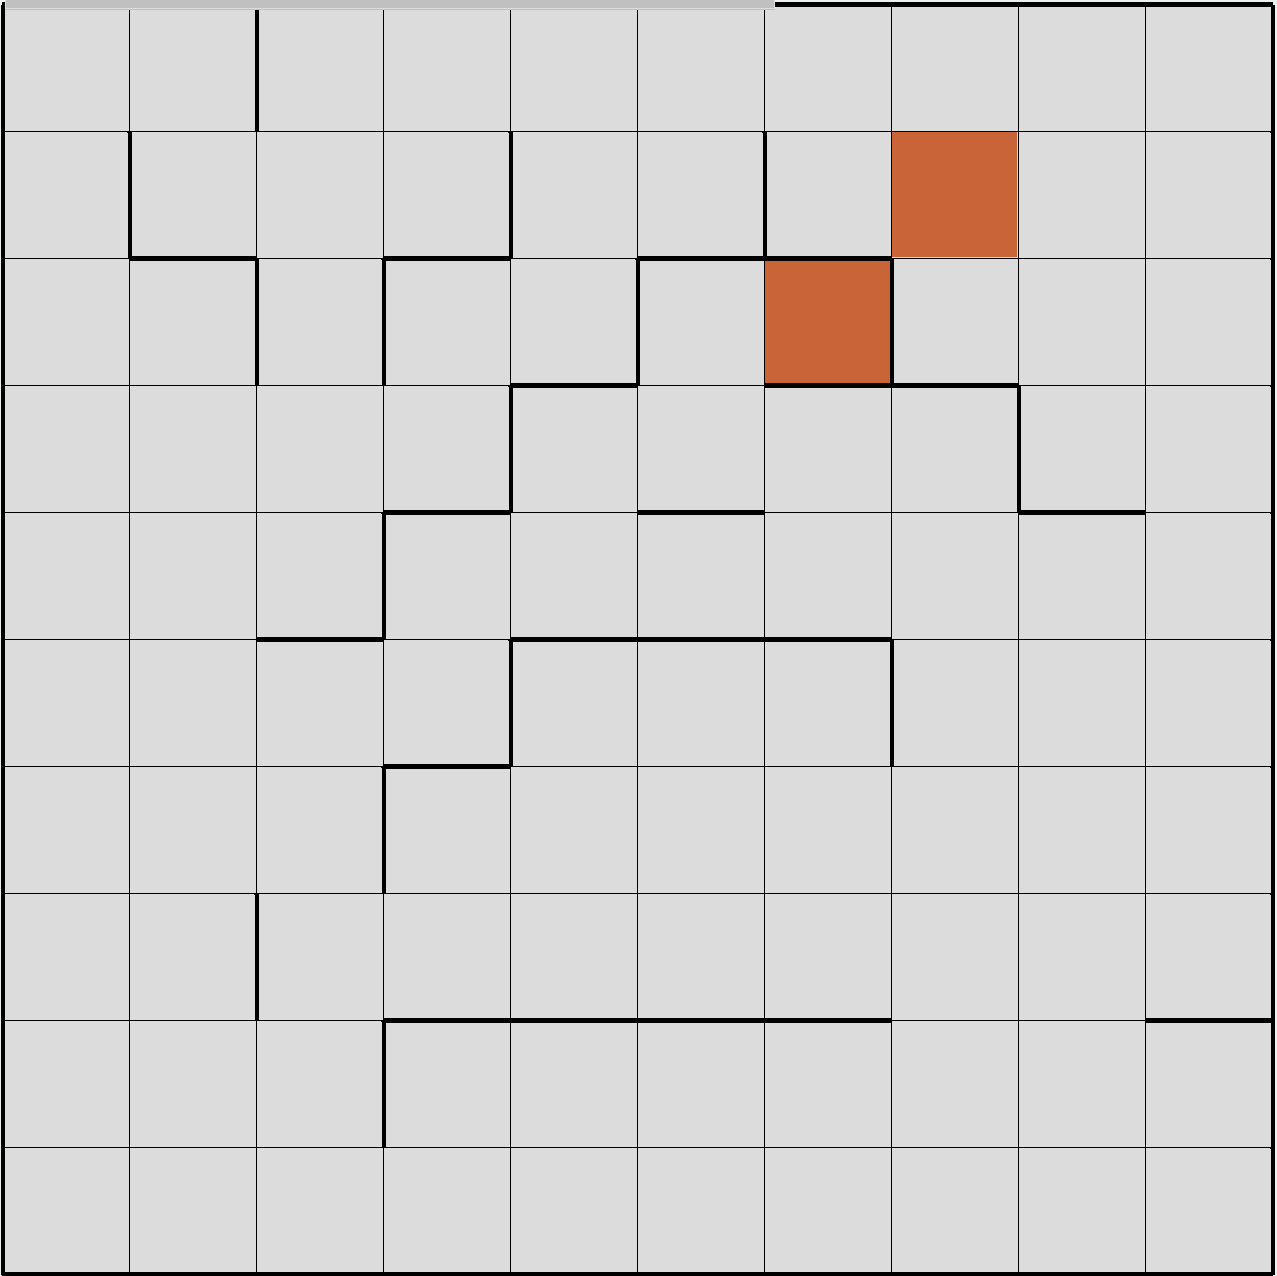
\includegraphics[width=1\linewidth]{../figures/maze2.png}
     \caption{Complex Maze}\label{Fig:maze2}
   \end{minipage}
\end{figure}\\
\\
In the figures, the highlighted grids are the destinations and the bold lines are walls and the agent cannot pass the wall. The possible actions for the agent are moving up, down, right or left and each action will have some constant cost. The parameter PJOG is the probability that the agent will act ineffectively. i.e. the agent will have 1-PJOG probability that its action will lead to the destination and PJOG/3 probability to choose other directions. Also, there would be some penalty if the agent tries to go into a wall.\\
\\
I believe these two problems are interesting. The first reason is that they can be mapped to some real life problems. For example, a robot has to go back to its charging position when its battery is low. Another reason is that I believe the problems can show the performance of different algorithms as well as help the selection of algorithms in different situations.
\section{Value Iteration}
For value iteration, it works by finding the optimal value function which can represent how good is a state for the agent.
\begin{table}[h!]
  \begin{center}
    \caption{Performance of Value Iteration}
    \label{Tab:value}
    \begin{tabular}{c|c|c|c|c}
      \textbf{PJOG} & \textbf{Small\_Steps} & \textbf{Small\_Time(ms)} & \textbf{Large\_Steps} & \textbf{Large\_Time(ms)}\\
      \hline
      0.1 & 24 & 4 & 42 & 40\\
      0.3 & 48 & 19 & 84 & 65\\
      0.5 & 123 & 23 & 181 & 143\\
    \end{tabular}
  \end{center}
\end{table}

\section{Policy Iteration}
\begin{table}[h!]
  \begin{center}
    \caption{Performance of Policy Iteration}
    \label{Tab:policy}
    \begin{tabular}{c|c|c|c|c}
			\textbf{PJOG} & \textbf{Small\_Steps} & \textbf{Small\_Time(ms)} & \textbf{Large\_Steps} & \textbf{Large\_Time(ms)}\\
      \hline
      0.1 & 5 & 40 & 6 & 92\\
      0.3 & 4 & 13 & 7 & 69\\
      0.5 & 4 & 24 & 5 & 100\\
    \end{tabular}
  \end{center}
\end{table}

\section{Comparison between Value Iteration and Policy Iteration}

\section{Q Learning}



\end{document}
